\documentclass{article}
\usepackage{graphicx,booktabs,longtable,amsmath}
\begin{document}
\chapter*{第 4 章　 大模型计算系统}


大语言模型（{Large Language Model}，LLM）的参数规模从数十亿到数千亿，训练和推理过程需要执行海量的张量运算，运行过程中还会不断产生激活值、梯度和缓存等中间状态。一个模型能否真正训练成功、能否以可接受的速度和成本响应用户请求，并不只取决于神经网络算法本身，还取决于承载它的整套计算系统：计算芯片负责执行矩阵运算，高带宽存储负责持续供给参数与缓存，互联网络负责在设备之间交换数据，软件框架负责把算法翻译成可执行的计算，推理服务和应用工具则把模型能力交付给最终用户。\textbf{大模型计算系统}就是由这些硬件与软件共同构成并相互配合的整体。

本章采用“需求—方案—效果”的思路展开。第\,4.1\,节首先回答“大模型对计算系统提出了哪些要求”，并给出几种简便的估算方法，由此引出计算系统的四层结构；第\,4.2～4.5\,节依次介绍各层的解决方案——算力资源、深度学习框架、推理服务和应用系统工具，并说明每种方案解决的问题及其代价；第\,4.6\,节通过一个完整的设计案例，把各层知识串联起来。

\begin{quote}

\par\textbf{学习目标}　{学完本章，读者应能够：}
\begin{enumerate}[leftmargin=2em]
  \item 用参数量、计算量和数据搬运量三个基本量，估算一个模型在训练或推理时对硬件的要求；
  \item 用算术强度和 Roofline 模型判断一项计算受算力限制还是受访存限制；
  \item 说明 CPU、GPU、NPU/ASIC 的分工，以及 HBM、NVLink、InfiniBand 分别作用于哪一段数据通路；
  \item 区分 CUDA 等计算软件栈、PyTorch 等深度学习框架与 vLLM、Ollama 等推理服务组件所处的层次；
  \item 估算训练显存与 KV 缓存，并据此选择分布式训练或推理优化手段；
  \item 综合考虑延迟、吞吐、显存、成本和工程复杂度，为一个具体应用设计合适的系统方案。
\end{enumerate}
\end{quote}

\section*{4.1　 大模型对计算系统提出的要求}


\begin{quote}

\noindent 动手选硬件、写代码之前，先要算清楚一笔账：大模型到底要计算多少、存储多少、搬运多少？本节用参数量 $N$、每个 token 的计算量和每次计算的数据搬运量做数量级估算，再借助 Roofline 模型判断瓶颈落在哪里。结论是：大模型同时受到算力、存储容量、存储带宽和设备互联四方面约束，计算系统的四层结构正是由此而来。
\end{quote}

\subsection*{4.1.1　 两个典型场景}

先看两个场景。

\textbf{场景一：训练。}某团队希望用 $2\times10^{12}$ 个 token 的语料，从头训练一个 70 亿参数（7B）的模型。他们需要知道：单张显卡的显存能否容纳模型？训练需要多长时间？需要多少张显卡？

\textbf{场景二：推理。}训练好的模型部署为在线问答服务，同时有上百名用户提问。服务方关心的是：用户需要等待多久才能看到第一个输出 token？每秒能输出多少个 token？一台服务器能同时服务多少用户？

这两个问题看似不同，背后却涉及同样的三个基本量：\textbf{存储量}（模型与中间状态占多少字节）、\textbf{计算量}（需要多少次浮点运算）和\textbf{数据搬运量}（运算时要在存储与计算单元之间移动多少字节）。下面逐一估算。

\subsection*{4.1.2　 三个基本量的估算}


\paragraph{存储量} 设模型有 $N$ 个参数，每个参数用 $b$ 位表示，则仅权重就至少占用
\[
M_{\mathrm{weight}} = \frac{N\,b}{8}\ \text{字节}. \tag{4-1}
\]
7B 模型若以 16 位浮点数（FP16 或 BF16）存储，需要 $7\times10^{9}\times 2 = 14\times10^{9}$ 字节，约 \SI{14}{GB}；若量化为 4 位，仅权重约 \SI{3.5}{GB}。训练时还要额外保存梯度和优化器状态，所需存储往往是权重本身的数倍（详见第\,4.3.3\,小节）。

\paragraph{计算量} 对于 Transformer 结构的模型，处理一个 token 的前向计算约需 $2N$ 次浮点运算（每个参数参与一次乘法和一次加法）；训练时还要做反向传播，计算量约为前向的两倍，因此每个训练 token 合计约 $6N$ 次浮点运算\cite{kaplan2020scaling}。于是训练总计算量可估算为
\[
C_{\mathrm{train}} \approx 6\,N\,D, \tag{4-2}
\]
其中 $D$ 为训练 token 总数。

\begin{quote}
\textbf{例 4-1　 训练需要多少张卡}


按场景一，$C_{\mathrm{train}}\approx 6\times7\times10^{9}\times2\times10^{12}=8.4\times10^{22}$ 次浮点运算。一张数据中心级 GPU 的 BF16 稠密峰值算力约为 $10^{15}$\,FLOP/s 量级（例如 NVIDIA H100 SXM 约 $9.9\times10^{14}$\,FLOP/s\cite{nvidia2023h100}）。实际训练中能达到峰值的 40\% 左右已属较高水平，即有效算力约 $4\times10^{14}$\,FLOP/s，则
\[
  t_{\text{单卡}} \approx \frac{8.4\times10^{22}}{4\times10^{14}} \approx 2.1\times10^{8}\ \text{s} \approx 6.7\ \text{年}.
\]
若使用 1024 张 GPU 并行训练，且并行效率理想，耗时可缩短到约 2.4 天。这说明：\textbf{大模型训练通常需要多卡乃至多机的分布式计算}，设备之间如何交换数据因此成为核心问题。
\end{quote}

\paragraph{数据搬运量} 计算单元只能处理已经送达的数据。推理时每生成一个新 token，都要把全部权重从显存读入计算单元一次：对于 \SI{14}{GB} 权重的 7B 模型，就意味着每个 token 至少读取 \SI{14}{GB} 数据。若显存带宽为 \SI{3.35}{TB/s}，则单个请求逐 token 生成的速度上限约为
\[
  \frac{3.35\times10^{12}\ \text{B/s}}{14\times10^{9}\ \text{B/token}} \approx 240\ \text{token/s}.
\]
该上限主要不由芯片峰值算力决定，而由\textbf{存储带宽}决定。可见，衡量计算系统时不能只看算力，还必须同时考察数据供给是否及时。

\subsection*{4.1.3　 瓶颈判断工具：算术强度与 Roofline 模型}


为判断一项计算究竟受算力限制还是受访存限制，引入\textbf{算术强度}（{arithmetic intensity}）：记一次计算的浮点运算次数为 $F$，需要在存储与计算单元之间搬运的字节数为 $Q$，则
\[
I = \frac{F}{Q}　(\text{FLOP/byte}). \tag{4-3}
\]
设硬件峰值算力为 $P_{\mathrm{peak}}$，存储带宽为 $B_{\mathrm{mem}}$。计算单元每秒最多完成 $P_{\mathrm{peak}}$ 次运算，而存储系统每秒最多供给 $B_{\mathrm{mem}}$ 字节数据、支撑 $I\cdot B_{\mathrm{mem}}$ 次运算，二者取较小者，即得 \textbf{Roofline 模型}\cite{williams2009roofline}给出的可达性能上界：
\[
P_{\mathrm{attainable}} \le \min\bigl(P_{\mathrm{peak}},\; I\cdot B_{\mathrm{mem}}\bigr). \tag{4-4}
\]
两条直线相交处的算术强度 $I^{*}=P_{\mathrm{peak}}/B_{\mathrm{mem}}$ 称为\textbf{拐点}。$I<I^{*}$ 时性能受带宽限制，称为\textbf{访存受限}（{memory-bound}）；$I>I^{*}$ 时性能受峰值算力限制，称为\textbf{计算受限}（{compute-bound}）。以前述 GPU 为例，$I^{*}\approx 9.9\times10^{14}/3.35\times10^{12}\approx 295$\,FLOP/byte。

\begin{figure}
\centering
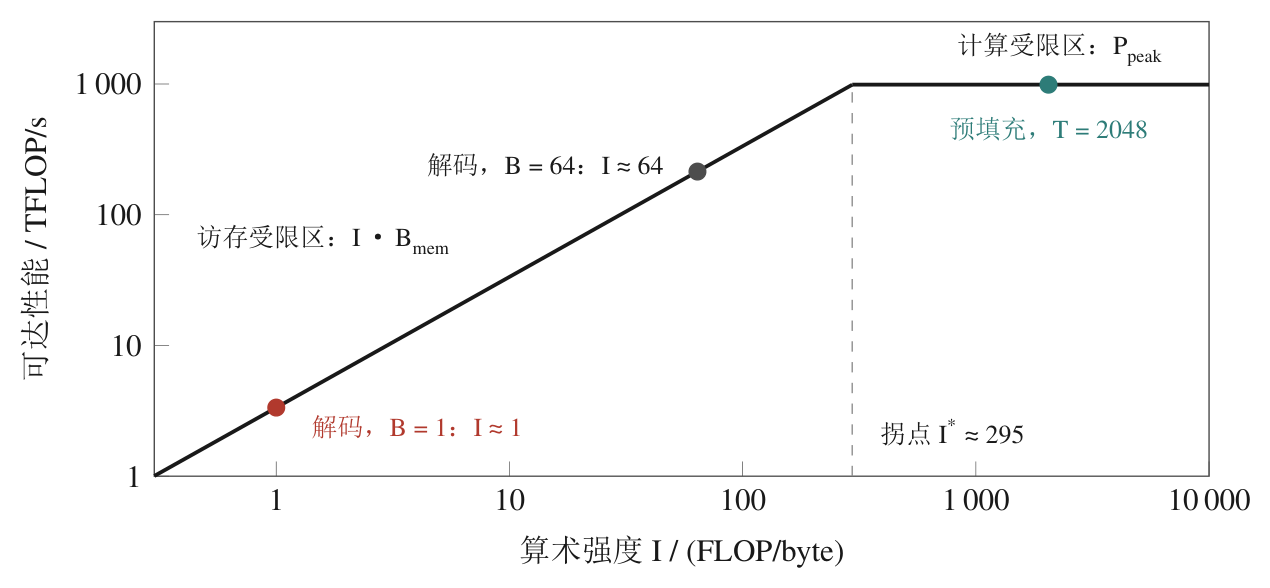
\includegraphics[width=0.9\linewidth]{figs/fig01.png}
\caption{图 4-1　 Roofline 模型示意。以峰值算力约 \SI{989}{TFLOP/s}、显存带宽约 \SI{3.35}{TB/s} 的 GPU 为例；坐标为对数刻度，各点为数量级估计}
\end{figure}

将 Roofline 模型用于推理的两个阶段（图\,4-1），可以得到一个重要结论。读入一次 16 位权重（2 字节）后，若只为一个 token 做 2 次运算，算术强度约为 $1$\,FLOP/byte，远低于拐点；若一次读入后同时为 $T$ 个 token 复用，算术强度约为 $T$。因此：
\begin{itemize}
  \item \textbf{预填充}（一次性处理用户输入的全部 token，$T$ 可达数千）的算术强度高，通常\textbf{计算受限}；
  \item \textbf{逐 token 解码}（每步只生成一个 token）的算术强度很低，通常\textbf{访存受限}；把多个请求合并成批次（批大小为 $B$）可使算术强度提高到约 $B$。
\end{itemize}
这就解释了一个常见现象：同一张显卡处理长输入（预填充阶段）时吞吐较高，而逐 token 解码时吞吐却较低——原因不是算力不足，而是每生成一个 token 都要重新读取大量权重和缓存。第\,4.4\,节介绍的许多推理优化技术，正是围绕这一点展开的。

\begin{quote}
\textbf{辨析}　 
Roofline 模型给出的是性能\textbf{上界}，不能用来精确预测实际性能。它的价值在于快速判断主要瓶颈：对访存受限的任务，提升峰值算力作用有限；对计算受限的任务，提升带宽同样作用有限。
\end{quote}

\subsection*{4.1.4　 从需求到方案：计算系统的四层结构}


综合以上估算，大模型对计算系统的需求可以归纳为四条：
\begin{enumerate}
  \item \textbf{算得快}——提供足够的浮点算力，并让算力被充分利用；
  \item \textbf{存得下、送得及}——有足够的存储容量容纳权重和中间状态，并有足够的带宽及时供给数据；
  \item \textbf{传得动}——当一张卡不够用时，多张卡、多台机器之间能高效交换数据；
  \item \textbf{用得上}——开发者能方便地表达模型、训练模型，用户能方便地调用模型。
\end{enumerate}

没有哪一个部件能单独满足这四条需求，于是形成了层次化的解决方案（图\,4-2）：底层的\textbf{算力资源}（芯片、存储、互联）提供物理能力；\textbf{驱动与计算软件栈}把硬件能力开放为可编程接口；\textbf{训练与推理框架}让开发者用张量运算表达模型，并自动完成求导、并行与调度；最上层的\textbf{应用系统工具}把模型组装成可部署、可管理的产品。每一层都向上层隐藏下层的复杂性，同时受到下层能力的约束。

\begin{figure}
\centering
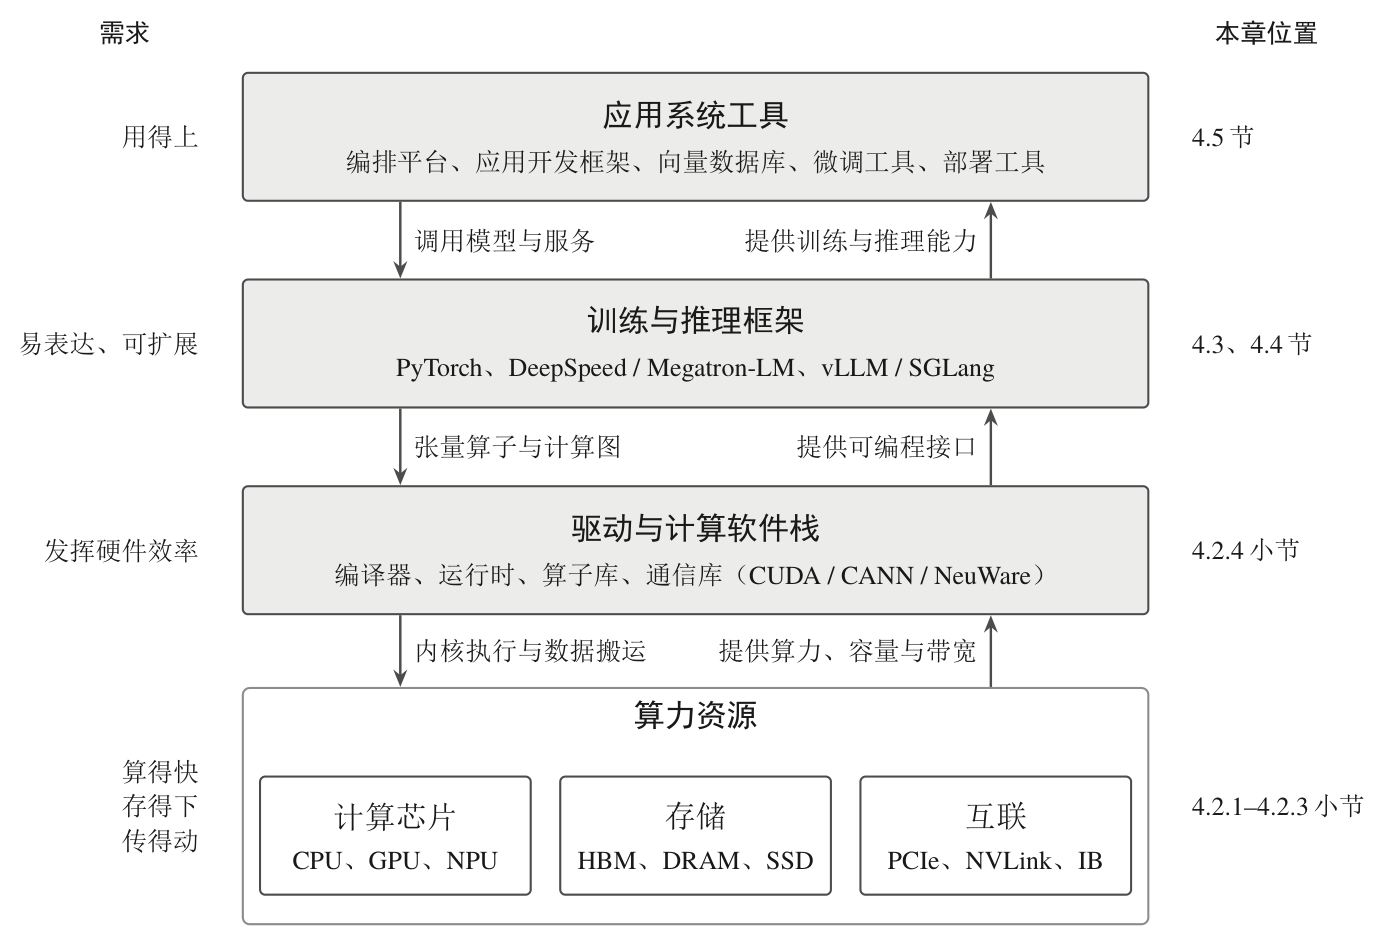
\includegraphics[width=0.9\linewidth]{figs/fig02.png}
\caption{图 4-2　 大模型计算系统的四层结构。左侧为各层满足的需求，右侧为对应的章节；向下的箭头表示上层向下层提交的工作，向上的箭头表示下层向上层提供的能力}
\end{figure}

表\,4-1 给出了本章各节与这四层结构的对应关系。阅读时可以随时回到图\,4-2，确认当前内容处在哪一层、解决的是哪一类需求。

\begin{table}[htbp]
\centering
\caption{表 4-1　 本章内容与系统层次的对应关系}

\begin{tabular}{l l l}
\toprule
节 & 所处层次 & 回答的核心问题 \\
\midrule
4.2　 算力资源 & 算力资源、驱动与软件栈 & 计算在哪里执行？数据如何存取和传输？ \\
4.3　 深度学习框架 & 训练与推理框架 & 如何方便地表达模型？单卡放不下时如何训练？ \\
4.4　 推理服务 & 训练与推理框架 & 如何让模型又快又省地回答大量请求？ \\
4.5　 应用系统工具 & 应用系统工具 & 如何把模型变成可使用、可管理的产品？ \\
4.6　 综合案例 & 全部层次 & 面对一个具体需求，如何自上而下地完成选型？ \\
\bottomrule
\end{tabular}
\end{table}

\section*{4.2　 算力资源：让计算算得快、存得下、传得动}


\begin{quote}


\noindent 上一节的估算给出了三项硬要求：高算力、大容量高带宽的存储，以及高速互联。硬件如何满足它们？计算芯片提供算力，HBM 等存储提供容量与带宽，NVLink、InfiniBand 等互联技术把多卡多机连成整体，驱动与计算软件栈再把这些能力开放给上层软件。不过要记住，硬件只决定性能的上界，能否接近上界，还要看软件能否用好它。


\end{quote}

\subsection*{4.2.1　 计算芯片：CPU、GPU 与 NPU/ASIC}


先看大模型到底在算什么。无论是注意力中的投影、注意力分数与加权求和，还是前馈网络中的两次线性变换，Transformer 的绝大部分计算都可以归结为矩阵乘法。矩阵乘法由海量彼此独立的乘加运算组成，谁先算、谁后算都不影响结果。因此，决定速度的不是单个运算有多快，而是\textbf{同一时刻能有多少运算并行进行}——大模型需要的是高并行吞吐，而不是单个任务的低延迟。

哪种芯片能提供这样的吞吐？不同芯片在“通用性”与“专用效率”之间做出了不同取舍（图\,4-3）。
\begin{itemize}
  \item \textbf{CPU}（{Central Processing Unit}，中央处理器）核心数较少，但每个核心具有复杂的分支预测和多级缓存，擅长控制流密集、需要低延迟响应的通用任务。在大模型系统中，CPU 通常负责操作系统、数据预处理、请求编排、内存管理，以及向加速器下发计算任务。
  \item \textbf{GPU}（{Graphics Processing Unit}，图形处理器）集成了成千上万个并行执行单元，并配有专门的矩阵乘加单元（如 NVIDIA 的 Tensor Core）和高带宽显存，适合训练和推理中的大规模线性代数运算\cite{hwu2026pmpp}。
  \item \textbf{NPU}（{Neural Processing Unit}，神经网络处理器）泛指为神经网络计算专门优化的处理器；\textbf{ASIC}（{Application-Specific Integrated Circuit}，专用集成电路）则泛指为特定用途定制设计的芯片。二者并非互斥的分类——前者按\textbf{用途}命名，后者按\textbf{实现方式}命名，一款 NPU 完全可以用 ASIC 方式实现。Google TPU、华为昇腾 NPU 和寒武纪 MLU 都属于这一类。
\end{itemize}

\begin{figure}
\centering
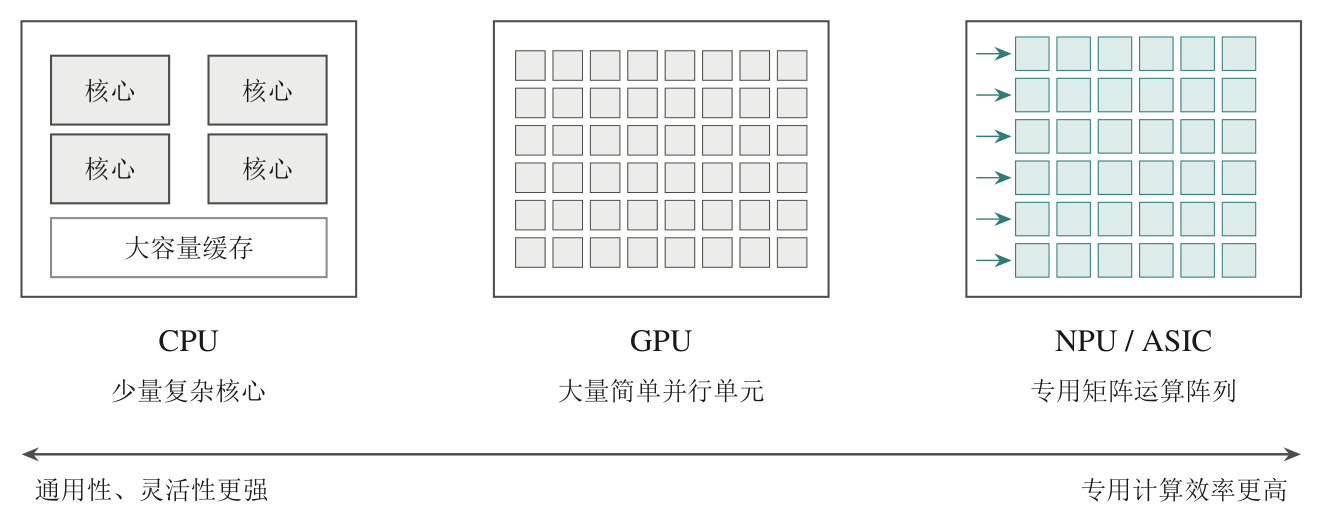
\includegraphics[width=0.9\linewidth]{figs/fig03.png}
\caption{图 4-3　 三类计算芯片的结构取舍（示意）。从左到右，芯片的通用性逐渐降低，矩阵运算的吞吐与能效逐渐提高}
\end{figure}

实际系统中，CPU 与加速器是\textbf{协同}关系而非替代关系：CPU 负责发起和调度，GPU 或 NPU 负责执行吞吐密集的张量运算。表\,4-2 对几类芯片做了概括。

\begin{table}[htbp]
\centering
\caption{表 4-2　 计算芯片的适用性比较}

\begin{tabular}{l l l l}
\toprule
类型 & 典型优点 & 典型限制 & 在大模型系统中的职责 \\
\midrule
CPU & 控制灵活，软件生态成熟 & 张量吞吐远低于专用加速器 & 预处理、调度、系统服务、小模型推理 \\
GPU & 并行吞吐高，深度学习生态成熟 & 显存容量有限，多卡互联成本高 & 训练、微调、高吞吐推理 \\
NPU / ASIC & 针对矩阵和低精度运算优化，能效高 & 框架、算子与驱动的兼容性因平台而异 & 云端或边缘侧的专用 AI 计算 \\
FPGA & 可重构，可定制数据通路 & 开发难度大，生态不如 GPU & 特定低延迟或定制化场景 \\
\bottomrule
\end{tabular}
\end{table}

专用化换来了更高的吞吐与能效，代价又是什么？一是通用性下降，二是软件生态的绑定加深。这也提醒我们，选择芯片时不能只比较“TFLOPS”或“TOPS”一个数字：不同精度（FP16、BF16、FP8、INT8）、是否计入稀疏加速，测得的峰值差别可达数倍。更可靠的做法是同时比较目标模型的支持情况、低精度格式、板载存储容量、编译器与算子库的成熟度、框架适配、集群通信能力，以及采购和运维成本。

\subsection*{4.2.2　 存储层次：为什么 HBM 如此重要}


第\,4.1.2\,小节留下了一个结论：解码时，每生成一个 token 都要把全部权重从显存读一遍，速度上限由显存带宽决定。训练时情况更紧张——权重、梯度、优化器状态和激活值都要驻留在设备上。于是存储系统要同时回答两个问题：\textbf{装不装得下}，以及\textbf{送不送得及}。

单一一种存储无法同时做到又大、又快、又便宜，计算机的办法是\textbf{分层}（图\,4-4）。越靠近计算单元，存储越快、越小、越贵：片上 SRAM（寄存器、共享内存、缓存）带宽最高但容量只有数十 MB；板载显存容量为数十 GB；主机内存（DRAM）可达 TB 级，但 GPU 访问它要经过 PCIe，带宽比显存低一个数量级以上；SSD 用于存放模型文件和冷数据。

\begin{figure}
\centering
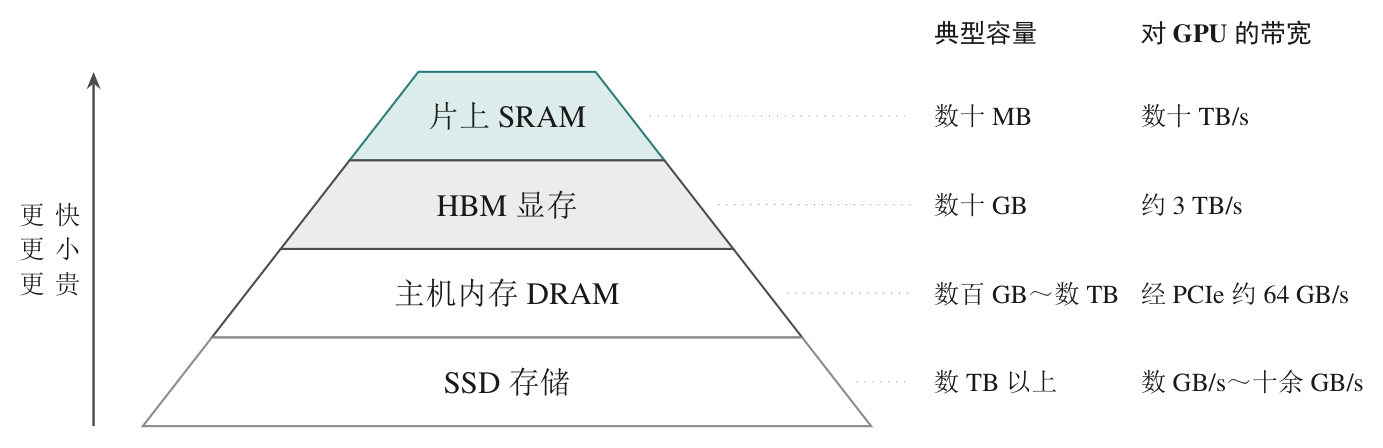
\includegraphics[width=0.9\linewidth]{figs/fig04.png}
\caption{图 4-4　 加速器视角下的存储层次（数量级示意，以 H100 级数据中心 GPU 为参照）。模型权重和 KV 缓存主要驻留在 HBM 中，计算时被反复读入片上 SRAM}
\end{figure}

在这个层次中，显存这一级对大模型最为关键，而\textbf{高带宽内存}（{High Bandwidth Memory}，HBM）是当前数据中心加速器的主流显存方案。它把多层 DRAM 芯片垂直堆叠，用\textbf{硅通孔}（{Through-Silicon Via}，TSV）实现层间互联，再通过很宽的接口（每个堆栈 1024 位）与计算芯片封装在一起。接口宽、距离短，使 HBM 能在有限的功耗和面积内提供远高于 GDDR 等传统显存的带宽。例如 H100 SXM 配备 \SI{80}{GB} HBM3，带宽约 \SI{3.35}{TB/s}\cite{nvidia2023h100}。

不过，HBM 解决的主要是“送不送得及”，而不是“装不装得下”。它价格昂贵，容量依然有限；运行大模型也并非必须使用 HBM——消费级显卡的 GDDR 显存同样可以运行规模适中或经过量化的模型。不妨把三个指标的分工记在一起：\textbf{容量决定模型和状态能否装下，带宽决定数据能否及时送达，延迟影响细粒度访问的效率}。

\begin{quote}
\textbf{辨析}　 
“7B 模型 4 位量化后仅权重就约 \SI{3.5}{GB}”不等于“有 \SI{4}{GB} 显存就能运行”。实际运行还需要存放量化缩放系数等元数据、KV 缓存、运行时缓冲区和临时张量，并存在内存碎片。估算时应在权重之外预留足够余量。
\end{quote}

\subsection*{4.2.3　 互联技术：PCIe、NVLink 与 InfiniBand}


一张卡总有装不下、算不完的时候。例\,4-1 表明，大模型训练需要成百上千张卡协同工作；即使只做推理，较大的模型也常常要切分到多张卡上。一旦切分，卡与卡之间就要不断交换梯度、激活值和中间结果。此时计算单元再快，如果数据迟迟不到，也只能空等。

讨论互联时，最有用的问题不是“哪种技术更快”，而是“\textbf{数据要从哪里传到哪里}”。不同层级的链路各有分工（图\,4-5）：
\begin{itemize}
  \item \textbf{PCIe}（{PCI Express}）是通用的设备互联总线，连接 CPU 与 GPU、网卡、NVMe 硬盘等外设。PCIe 5.0 x16 的单向带宽约 \SI{64}{GB/s}。
  \item \textbf{NVLink} 是 NVIDIA 的 GPU 高速互联技术，用于同一服务器内 GPU 与 GPU（或与 Grace CPU）之间的直接通信，带宽远高于 PCIe（H100 每卡 NVLink 总带宽约 \SI{900}{GB/s}\cite{nvidia2023h100}）。配合 NVSwitch 交换芯片，可以让一台服务器内的 8 张 GPU 两两全速互联。
  \item \textbf{InfiniBand}（IB）是面向高性能计算集群的\textbf{跨节点}网络，单端口带宽可达 \SI{400}{Gb/s}（NDR）。它原生支持 \textbf{RDMA}（{Remote Direct Memory Access}，远程直接内存访问）：数据可以直接写入远端机器的内存，而不必经过双方 CPU 的多次拷贝和内核协议栈处理。以太网借助 \textbf{RoCE}（{RDMA over Converged Ethernet}）也能实现 RDMA，成本较低，但在拥塞控制和延迟稳定性上通常需要更细致的调优。
\end{itemize}

\begin{figure}
\centering
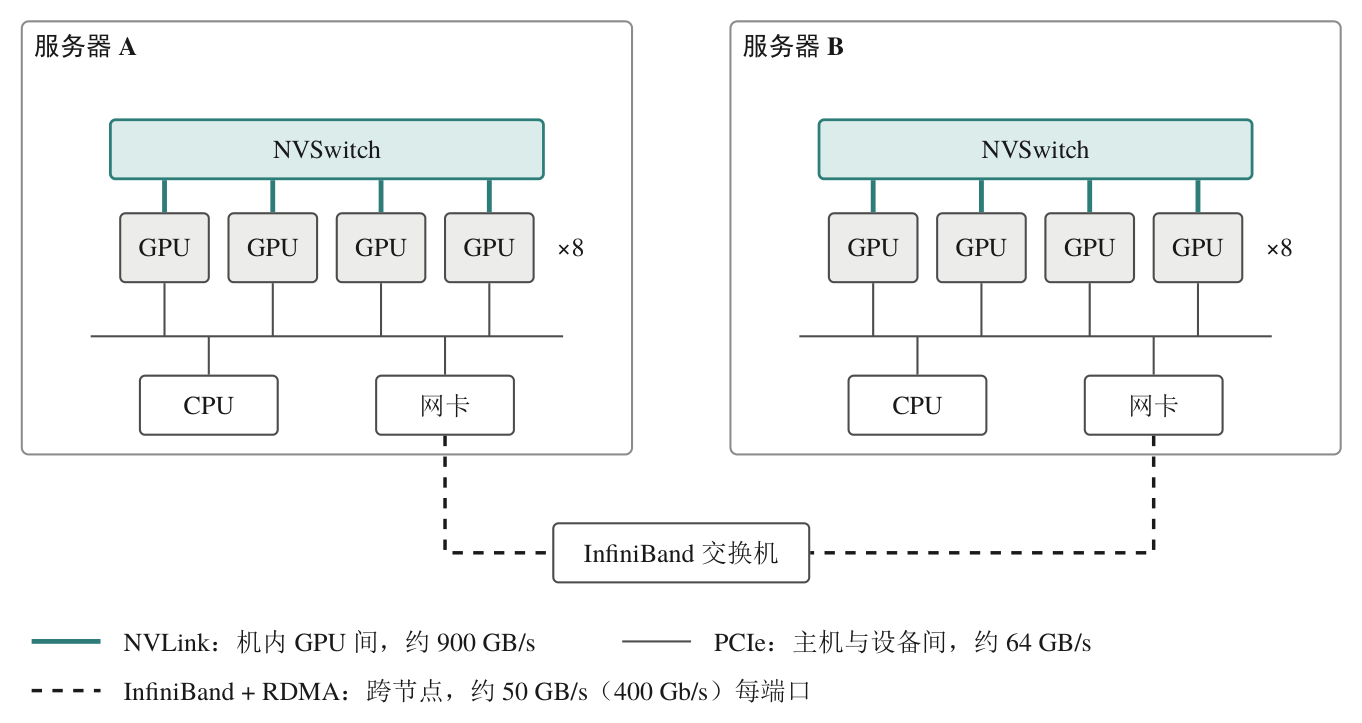
\includegraphics[width=0.9\linewidth]{figs/fig05.png}
\caption{图 4-5　 单机内与跨节点的典型数据通路（示意）。机内 GPU 经 NVLink/NVSwitch 互联，GPU 与 CPU、网卡之间经 PCIe 连接，不同服务器之间经 InfiniBand 网络通信。带宽为 H100 一代硬件的数量级参考值，具体取决于配置}
\end{figure}

把这几个数字放在一起，就能看出一条规律：不同层级链路的带宽相差一个数量级以上，因此\textbf{通信越频繁的工作，越应该放在越近的地方}。第\,4.3.4\,小节会看到，张量并行每一层都要通信，应当留在 NVLink 相连的同一台机器内；数据并行、流水线并行通信较少，才适合跨越 InfiniBand 网络。也正因为二者位于不同的互联层级、解决不同的问题，NVLink 与 InfiniBand 不应混为一谈。

\begin{quote}
\textbf{辨析}　 
“RDMA 完全绕过操作系统”只是一种简化说法。实际使用 RDMA 仍需注册内存、加载驱动、管理权限与连接；更准确的表述是：RDMA \textbf{在数据传输路径上}省去了常规的 CPU 数据拷贝和部分内核协议处理，从而降低延迟和 CPU 开销。
\end{quote}

\subsection*{4.2.4　 驱动与计算软件栈：CUDA、CANN 与 NeuWare}


有了芯片、存储和互联，还差最后一环：硬件只能执行机器指令，而算法开发者写的是 \texttt{torch.matmul} 这样的高层算子，谁来完成两者之间的翻译？答案是一套软件，它负责把高层算子翻译成设备上可执行的\textbf{内核}（{kernel}），并管理设备内存、任务调度和多卡通信。

这套软件称为\textbf{计算软件栈}，通常包括驱动、运行时、编译器、算子库和集合通信库五部分。以一次矩阵乘法为例（图\,4-6）：框架收到 \texttt{matmul} 调用后选择具体实现；算子库（或编译器生成的代码）提供针对该硬件优化的内核；运行时负责分配显存、启动内核和同步；驱动把命令提交给硬件执行。多卡训练时，集合通信库负责完成 All-Reduce 等跨设备数据交换。

\begin{figure}
\centering
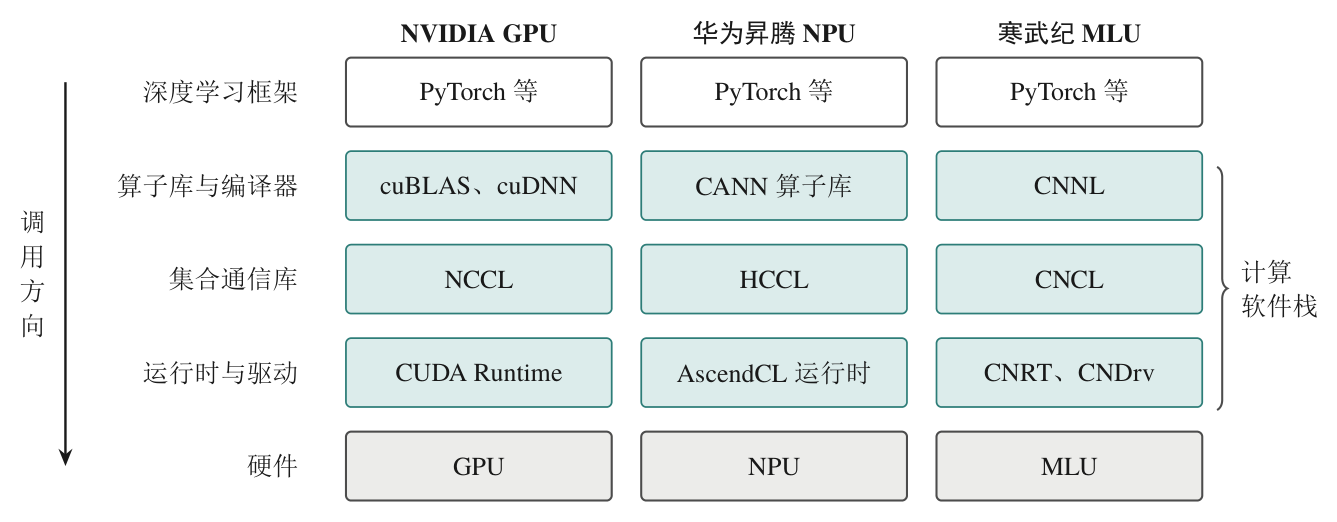
\includegraphics[width=0.9\linewidth]{figs/fig06.png}
\caption{图 4-6　 计算软件栈的层次与三种平台的对应组件。一次矩阵乘法调用自上而下依次经过各层；不同平台的组件职责相似，但实现与行为并不完全等价}
\end{figure}

不同硬件平台各有自己的软件栈：
\begin{itemize}
  \item \textbf{CUDA} 是 NVIDIA 面向自家 GPU 的并行计算平台和编程模型，包括编程接口、编译器、运行时，以及 cuBLAS（线性代数）、cuDNN（深度学习算子）、NCCL（集合通信）等库\cite{nvidia2024cuda}。经过近二十年积累，CUDA 生态是当前大模型训练与推理最主要的底层基础。
  \item \textbf{CANN} 是华为昇腾 NPU 的异构计算架构，提供编译器、运行时、算子库和 HCCL 集合通信库，承担与 CUDA 类似的职责。
  \item \textbf{NeuWare} 是寒武纪 MLU 系列芯片的基础软件平台，同样包含编程接口、编译工具与基础算子库。
\end{itemize}

软件栈的成熟程度，决定了硬件峰值性能能够发挥出多少。同一个模型在不同平台上的性能、算子支持范围和调试方法之所以不同，根源往往就在这一层。可见，CANN 等软件栈并非“PyTorch 的一个插件”；即使接口名称相似，也不能想当然地认为所有算子的行为和精度完全一致，迁移模型时需要逐项验证。

\begin{quote}
\textbf{本节要点}


\begin{itemize}[leftmargin=1.5em]
  \item 芯片提供算力，存储提供容量与带宽，互联技术连接多卡多机，软件栈把硬件能力开放给上层。
  \item 判断硬件是否合适，要同时看算力、显存容量、显存带宽、互联拓扑和软件生态，而非单一峰值指标。
  \item 并行策略应与互联拓扑相匹配：通信越频繁的切分，越应放在带宽越高的链路上。
\end{itemize}
\end{quote}

\section*{4.3　 深度学习框架：把算法组织成可执行的计算}


\begin{quote}


\noindent 有了硬件，开发者并不想为每种芯片手写内核、手工推导梯度；模型大到单卡装不下时，也不想从头处理多卡通信。深度学习框架正是为此而生：通用框架（如 PyTorch）提供张量、自动微分、优化器和设备管理，大模型训练框架（如 DeepSpeed、Megatron-LM）在其上增加并行切分与状态分片。这样，同一份模型代码就能在不同硬件和规模下运行，显存与通信的开销也可以事先用公式估算，并据此选择并行策略。


\end{quote}

\subsection*{4.3.1　 为什么需要深度学习框架}

深度学习模型由许多层组成，每一层又包含矩阵乘法、激活函数、归一化等基本运算。这些基本运算在不同模型之间高度共性。如果每实现一个新模型都要直接编写设备内核、手工推导梯度，开发成本将难以承受，代码也无法在不同硬件间复用。

\textbf{深度学习框架}把这些共性运算封装成标准化组件——张量、算子、自动微分、优化器、设备调度、模型模块和分布式通信——供开发者组合使用\cite{zhang2023d2l}。这种封装带来两方面的好处：算法开发者能够快速表达和修改模型；系统开发者则可以集中精力，针对具体硬件优化少数热点算子，让所有上层模型同时受益。

使用框架训练一个模型的典型流程是：用张量运算定义模型与损失函数；框架根据计算图自动求出损失对各参数的梯度；优化器按学习率等规则更新参数；所有计算交由下层软件栈和硬件执行。表\,4-3 列出了几类代表性框架。

\begin{table}[htbp]
\centering
\caption{表 4-3　 代表性深度学习框架}

\begin{tabular}{l l l}
\toprule
类别 & 代表 & 定位 \\
\midrule
通用框架 & PyTorch、TensorFlow & 张量计算与自动微分，开发灵活，生态完整 \\
大模型训练框架 & DeepSpeed、Megatron-LM & 基于 PyTorch 扩展，提供大规模并行训练与显存优化 \\
推理框架 & vLLM、SGLang & 面向大模型推理服务，侧重缓存管理与请求调度（见第\,4.4\,节） \\
\bottomrule
\end{tabular}
\end{table}

\subsection*{4.3.2　 PyTorch：张量、自动微分与编译优化}


PyTorch 由 Facebook AI Research（现 Meta AI）于 2017 年开源，前身是 2002 年发布、以 Lua 为接口的 Torch 框架\cite{paszke2019pytorch}。它的三个核心概念是：

\paragraph{张量} \texttt{torch.Tensor} 是多维数组，可以存放在 CPU 或 GPU 等设备上，支持类似 NumPy 的运算接口。

\paragraph{自动微分} PyTorch 的 Autograd 系统在前向计算时记录各运算之间的依赖关系，形成\textbf{计算图}；调用 \texttt{backward()} 时，按链式法则从损失出发反向计算每个参数的梯度。以线性层 $\boldsymbol{y}=W\boldsymbol{x}+\boldsymbol{b}$ 和平方误差损失 $\mathcal{L}=\tfrac12\lVert\boldsymbol{y}-\boldsymbol{t}\rVert_2^2$ 为例，由链式法则可得
\[
\frac{\partial\mathcal{L}}{\partial W} = (\boldsymbol{y}-\boldsymbol{t})\,\boldsymbol{x}^{\top},\qquad
  \frac{\partial\mathcal{L}}{\partial \boldsymbol{b}} = \boldsymbol{y}-\boldsymbol{t}. \tag{4-5}
\]
框架并不显式求解参数，它只是按链式法则计算梯度，再由优化器据此迭代更新参数。大型 Transformer 的训练遵循完全相同的逻辑，只是计算图更大、算子更多。

\paragraph{动态图与编译} PyTorch 默认采用\textbf{动态图}（{eager execution}）：代码逐行执行，计算图在运行时随之构建，因此可以直接使用 Python 的条件与循环，也便于调试。代价是每个算子都要经过 Python 解释器调度，难以做跨算子的全局优化。PyTorch 2.x 引入了 \texttt{torch.compile}，可以在运行时捕获计算图，进行算子融合等优化后再编译执行，兼顾动态图的灵活性与静态图的性能\cite{ansel2024pytorch2}。

下面是一个完整训练步骤的最小示例，对应上述三个概念：

\begin{lstlisting}[language=Python]
import torch
model = torch.nn.Linear(1024, 1024).to("cuda")    # 张量与模块放到 GPU
opt = torch.optim.AdamW(model.parameters(), lr=1e-4)
model = torch.compile(model)                       # 可选：图捕获与编译优化
x = torch.randn(32, 1024, device="cuda")
t = torch.randn(32, 1024, device="cuda")
loss = 0.5 * ((model(x) - t) ** 2).sum()           # 前向：记录计算图
loss.backward()                                    # 反向：自动求梯度
opt.step(); opt.zero_grad()                        # 优化器更新参数
\end{lstlisting}

\begin{quote}
\textbf{辨析}　 
\texttt{torch.compile} 并非在所有情况下都能加速。动态变化的张量形状、不受支持的算子、首次编译的耗时以及模型结构本身，都会影响最终收益。是否开启、收益多少，应以实测为准。
\end{quote}

\subsection*{4.3.3　 训练显存：一张卡要装下什么}


在决定是否需要分布式训练之前，先要回答一个更基本的问题：一张卡到底要装下什么？答案不只是权重，还包括梯度、优化器状态和激活值。

把它们逐项相加即可。设模型有 $N$ 个参数，每个参数的权重、梯度、优化器状态和主权重副本分别占 $b_w$、$b_g$、$b_o$、$b_m$ 字节，则全参数训练的显存近似为
\[
M_{\mathrm{train}} \approx N\,(b_w+b_g+b_o+b_m) + M_{\mathrm{act}} + M_{\mathrm{workspace}}, \tag{4-6}
\]
其中 $M_{\mathrm{act}}$ 为激活值占用，与批大小和序列长度成正比；$M_{\mathrm{workspace}}$ 为临时缓冲区。

\begin{quote}
\textbf{例 4-2　 7B 模型的训练显存}


当前大模型训练的常见配置是 BF16 混合精度加 Adam 优化器\cite{rajbhandari2020zero}：BF16 权重 2 字节、BF16 梯度 2 字节、FP32 主权重 4 字节、Adam 的一阶矩与二阶矩各 4 字节，合计 16 字节/参数。对于 $N=7\times10^9$，仅模型状态就需要
\[
  7\times10^{9}\times16 = 112\times10^{9}\ \text{字节} \approx \SI{112}{GB},
\]
尚未计入激活值。这已经超过单张 \SI{80}{GB} 显卡的容量。若改用 FP32 权重与梯度、带动量的 SGD（共 12 字节/参数），则约为 \SI{84}{GB}。
\end{quote}

可见，显存需求\textbf{不是模型的固有属性}，而取决于精度、优化器以及主权重副本的存储方式；引用或计算这类数字时必须说明前提。降低显存的手段主要有三类：混合精度与低精度优化器改变每参数字节数；\textbf{激活检查点}（{activation checkpointing}）在反向传播时重新计算部分中间结果，以额外计算换取激活显存的节省；\textbf{参数高效微调}（如 LoRA\cite{hu2021lora}）只训练少量新增参数，大幅减少梯度与优化器状态。当这些手段仍不够时，就需要把模型和状态\textbf{切分}到多张卡上。

\subsection*{4.3.4　 单卡放不下怎么办：分布式训练}


既然一张卡放不下，最直接的想法就是把模型和训练状态“切开”，分给多张卡。切分对象不同，就得到不同的并行方式（图\,4-7）：
\begin{itemize}
  \item \textbf{数据并行}（{Data Parallelism}，DP）：每张卡保存完整的模型副本，处理不同的小批量数据，反向传播后通过 All-Reduce 汇总梯度并同步更新。它能提高样本吞吐量，但\textbf{不减少}每张卡上的模型状态占用。
  \item \textbf{张量并行}（{Tensor Parallelism}，TP）：把同一层内部的矩阵按行或列切开，分给多张卡共同计算\cite{shoeybi2019megatron}。单卡显存需求随之下降，但每一层都要交换中间结果，通信非常频繁，因此张量并行通常只在 NVLink 互联的单机内使用。
  \item \textbf{流水线并行}（{Pipeline Parallelism}，PP）：把不同的层分配到不同的卡上，形成多个流水线阶段，并让多个微批次交错执行。流水线并行的通信量较小，主要挑战是各阶段负载不均，以及流水线启动和排空时产生的空闲时间（称为\textbf{流水线气泡}）。
  \item \textbf{专家并行}（{Expert Parallelism}，EP）：在混合专家（MoE）模型中把不同的专家放在不同的卡上，token 按路由结果通过 All-to-All 通信发往对应专家。
\end{itemize}

\begin{figure}
\centering
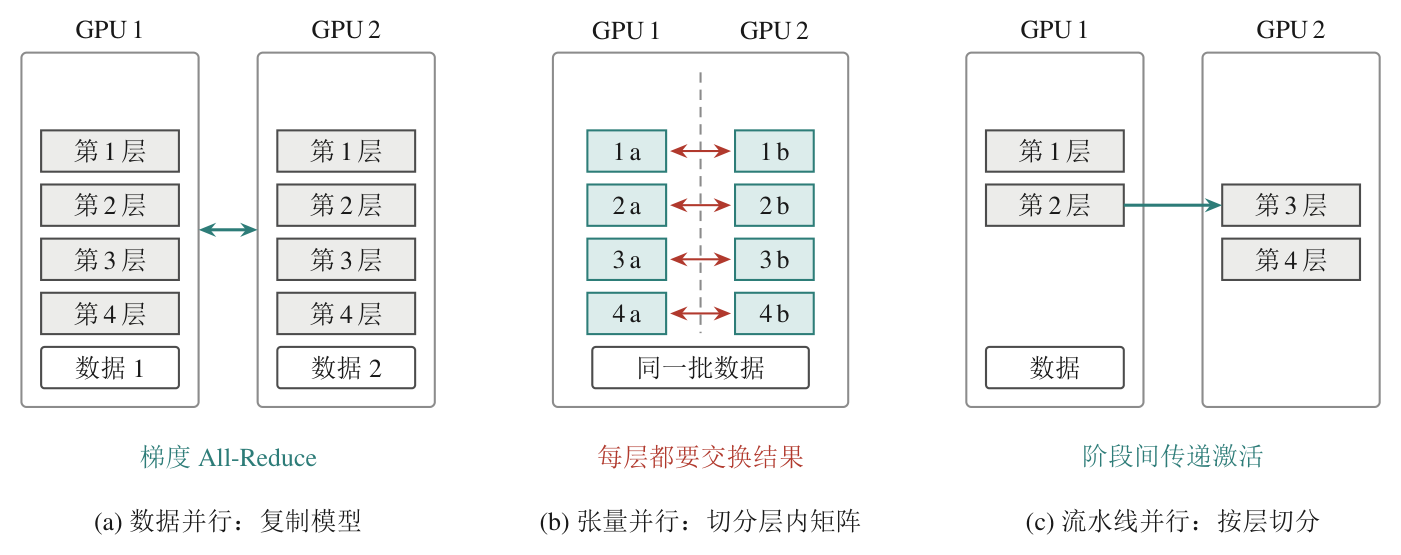
\includegraphics[width=0.9\linewidth]{figs/fig07.png}
\caption{图 4-7　 三种基本并行方式的切分对象（以 2 张 GPU、4 层模型为例）。红色箭头表示频繁通信，应放在高带宽链路上}
\end{figure}

数据并行的冗余问题可以通过\textbf{状态分片}来解决。DeepSpeed 的 ZeRO（{Zero Redundancy Optimizer}）\cite{rajbhandari2020zero}在数据并行的基础上，把模型状态切分到 $K$ 张卡上：第 1 阶段（ZeRO-1）只切分优化器状态；第 2 阶段（ZeRO-2）再切分梯度；第 3 阶段（ZeRO-3）连参数也一并切分，计算到某一层时才临时把完整参数收集回来。PyTorch 的 FSDP（{Fully Sharded Data Parallel}）提供了与 ZeRO-3 类似的功能。

状态分片究竟能省多少显存？以例\,4-2 中每参数 16 字节的配置为例，记优化器状态与主权重合计为 12 字节/参数，在 $K=8$ 张卡上，每张卡的模型状态显存分别为：
\begin{align*}
  \text{普通数据并行：} &\ (2+2+12)\,N = 16N, \\
  \text{ZeRO-1：} &\ (2+2+12/K)\,N = 5.5N, \\
  \text{ZeRO-2：} &\ (2+(2+12)/K)\,N = 3.75N, \\
  \text{ZeRO-3：} &\ (16/K)\,N = 2N.
\end{align*}
对于 7B 模型，对应约 112、38.5、26.3 和 \SI{14}{GB}（图\,4-8）。

\begin{figure}
\centering
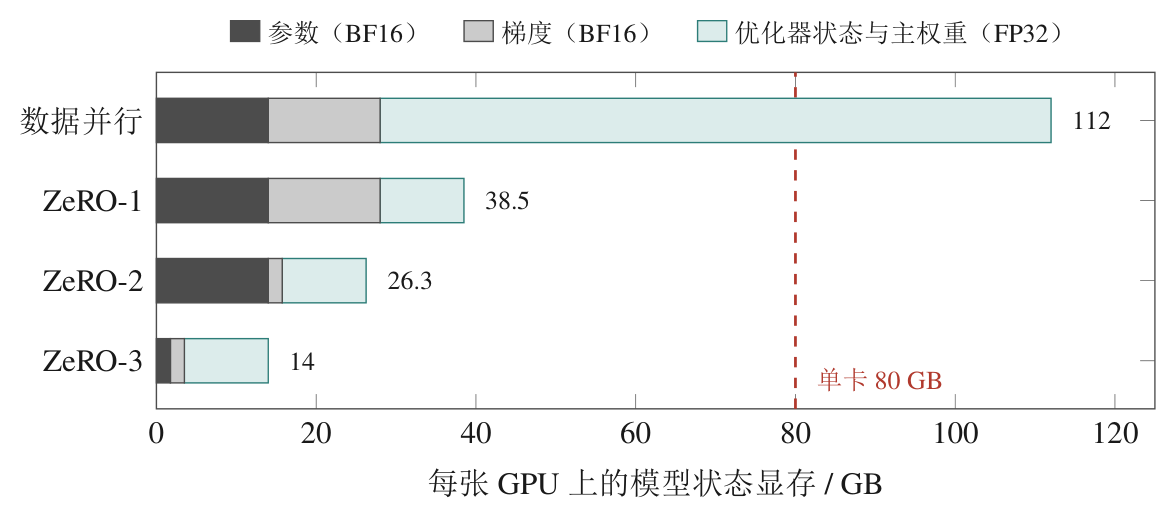
\includegraphics[width=0.9\linewidth]{figs/fig08.png}
\caption{图 4-8　 7B 模型在 8 张 GPU 上采用不同 ZeRO 阶段时，每张卡的模型状态显存（BF16 混合精度 + Adam，未计激活值与通信缓冲区）}
\end{figure}

省下的显存并不是免费的。分片越彻底，需要的通信也越多，例如 ZeRO-3 每计算一层都要先把完整参数收集回来。因此，理论上的显存节省比例不能直接等同于实际可用显存的增加或训练速度的提升。实际的大规模训练通常把数据并行、张量并行和流水线并行组合使用（常称为“3D 并行”）：机内用张量并行，机间用流水线并行，最外层再叠加数据并行或 ZeRO，使通信最频繁的切分落在带宽最高的链路上。

\subsection*{4.3.5　 训练系统的四类瓶颈}

把上述讨论归纳起来，大规模训练常遇到四类瓶颈，每一类都有相应的应对手段（表\,4-4）。

\begin{table}[htbp]
\centering
\caption{表 4-4　 大规模训练的四类瓶颈与应对手段}

\begin{tabular}{l l l}
\toprule
瓶颈 & 表现 & 主要应对手段 \\
\midrule
内存墙 & 模型状态与激活值放不下 & 混合精度、状态分片（ZeRO/FSDP）、激活检查点、参数高效微调 \\
计算墙 & 算子效率低，算力利用率不足 & 高效内核（如 FlashAttention）、算子融合、编译优化 \\
通信墙 & GPU 频繁等待数据传输 & 并行策略与拓扑匹配、通信与计算重叠、高速互联 \\
工程墙 & 配置复杂，故障频发，难以稳定运行 & 检查点保存与恢复、监控与日志、自动化调参工具 \\
\bottomrule
\end{tabular}
\end{table}

\begin{quote}
\textbf{本节要点}


\begin{itemize}[leftmargin=1.5em]
  \item 框架通过张量、自动微分和优化器，把“定义模型”与“执行计算”分离开来。
  \item 训练显存可按式\,\eqref{eq:train-mem} 估算；结果取决于精度与优化器，必须写明前提。
  \item 数据并行切分数据，张量并行切分层内矩阵，流水线并行切分层，ZeRO 切分模型状态；省显存往往以多通信为代价。
\end{itemize}
\end{quote}

\section*{4.4　 推理服务：让模型又快又省地回答请求}


\begin{quote}


\noindent 模型训练好之后，要面对的是真实用户：首字要出得快，输出要流畅，而显卡数量有限，还要尽量服务更多的人。从哪里入手？本节先把推理拆成预填充与解码两个阶段分别分析，再看 KV 缓存如何避免重复计算，以及 FlashAttention、PagedAttention、连续批处理和量化各自缓解哪一个瓶颈。效果用 TTFT、TPOT、吞吐和尾延迟等指标衡量；各项优化作用于不同环节，可以叠加使用，但彼此不能替代。


\end{quote}

\subsection*{4.4.1　 推理的两个阶段：预填充与解码}


大模型以\textbf{自回归}方式生成文本：每次只预测下一个 token，并把它追加到输入末尾，再预测下一个。据此，一次请求的处理可以分为两个阶段（图\,4-9）。

\paragraph{预填充（Prefill）} 模型一次性并行处理用户输入的全部 token，计算每一层的注意力 Key 与 Value 并保存下来，同时得到第一个输出 token。由于大量 token 共享同一次权重读取，这一阶段算术强度高，通常\textbf{计算受限}。衡量它的指标是\textbf{首 token 延迟}（{Time To First Token}，TTFT），即从发出请求到看到第一个输出 token 的时间，其中还包括请求排队的时间。

\paragraph{解码（Decode）} 模型逐个生成后续 token。每一步只处理一个新 token，却要读取全部权重和此前积累的 Key、Value，因此算术强度很低，通常\textbf{访存受限}（见第\,4.1.3\,小节）。衡量它的指标是\textbf{每 token 输出时间}（{Time Per Output Token}，TPOT），或其倒数——输出速度（token/s）。

\begin{figure}
\centering
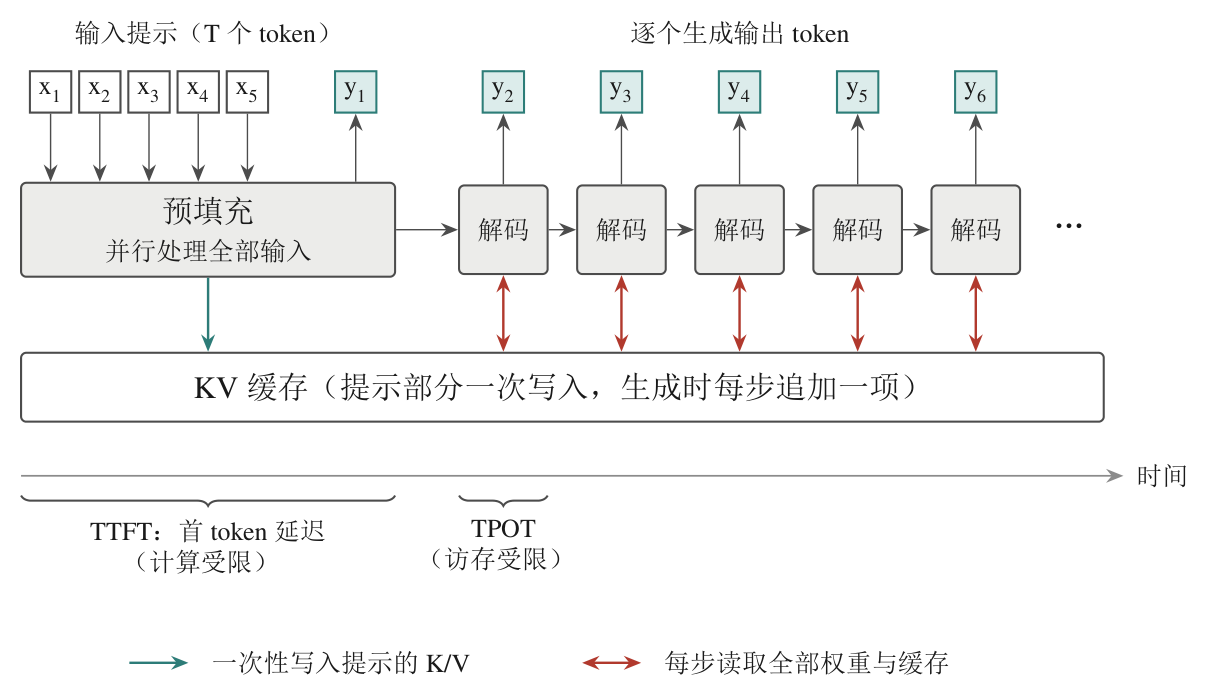
\includegraphics[width=0.9\linewidth]{figs/fig09.png}
\caption{图 4-9　 一次推理请求的两个阶段。预填充并行处理全部输入、写入 KV 缓存并给出首个 token；之后每个解码步只生成一个 token，却要读取全部权重与已有缓存}
\end{figure}

两个阶段的特性不同，优化方向也不同：输入越长，预填充越耗时，TTFT 越大；输出越长，解码步数越多，总生成时间越长。

\subsection*{4.4.2　 KV 缓存：用存储换计算}


进入解码阶段后，每个新 token 都要与之前所有 token 的 Key 和 Value 做注意力运算。如果每生成一个 token 都把全部历史 token 的 Key 和 Value 重新算一遍，总计算量将随序列长度呈平方增长。这种重复能否避免？

注意到历史 token 的 Key 和 Value 一旦算出就不会改变，因此可以把它们保存下来，每步只为新 token 计算一次并追加到缓存中。这就是 \textbf{KV 缓存}（{KV cache}）。需要强调的是，KV 缓存保存的是注意力计算所需的中间状态，而不是已经生成好的答案。

省下的计算要用显存来换。KV 缓存的大小可估算为
\[
M_{\mathrm{KV}} \approx 2 \times L \times H_{\mathrm{KV}} \times d_{\mathrm{head}} \times T \times B \times b_{\mathrm{KV}}, \tag{4-7}
\]
其中系数 2 对应 Key 和 Value，$L$ 为层数，$H_{\mathrm{KV}}$ 为 KV 头数，$d_{\mathrm{head}}$ 为每个头的维度，$T$ 为序列长度，$B$ 为同时驻留的请求数，$b_{\mathrm{KV}}$ 为每个元素的字节数。

\begin{quote}
\textbf{例 4-3　 KV 缓存与并发上限}


某 8B 模型有 32 层，采用分组查询注意力（GQA），KV 头数为 8，每头 128 维，以 BF16 存储（2 字节）。单个请求、序列长度 4096 时，
\[
  M_{\mathrm{KV}} = 2\times32\times8\times128\times4096\times1\times2 \approx 5.4\times10^{8}\ \text{字节} = \SI{0.5}{GiB}.
\]
在 \SI{80}{GB} 显卡上，BF16 权重约占 \SI{16}{GB}。即使不计其他开销，剩余显存也只能容纳约 $64/0.54\approx 119$ 个这样的请求。若序列长度增加到 32K，单个请求的 KV 缓存将达到 \SI{4}{GiB}，并发上限随之降至约 15 个。
\end{quote}

可见，KV 缓存随序列长度和并发数线性增长，往往比权重本身更早耗尽显存（图\,4-10），成为长上下文、高并发服务的主要约束。计算时要注意：采用 GQA 或 MQA（多查询注意力）的模型，$H_{\mathrm{KV}}$ 小于查询头数，不能误用查询头数代入。

\begin{figure}
\centering
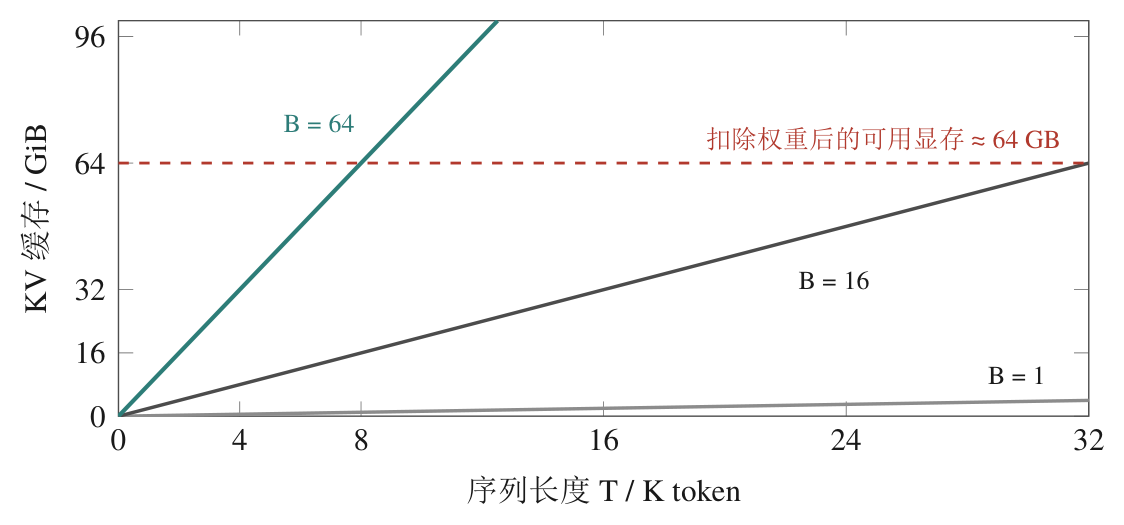
\includegraphics[width=0.9\linewidth]{figs/fig10.png}
\caption{图 4-10　 例\,4-3 中 8B 模型的 KV 缓存随序列长度 $T$ 与并发请求数 $B$ 的变化（BF16）。曲线与虚线的交点给出了该配置下能够支撑的最大上下文长度}
\end{figure}

\subsection*{4.4.3　 推理优化技术}


围绕上述瓶颈，形成了一系列推理优化技术。理解它们的关键，是分清每一种技术\textbf{作用于哪个环节、解决什么问题}。

\paragraph{FlashAttention：减少注意力计算中的显存读写} 标准注意力实现会把 $T\times T$ 的注意力分数矩阵完整写入显存再读回，序列越长，访存开销越大。FlashAttention\cite{dao2022flashattention}把计算分块，使中间结果尽量留在片上 SRAM 中，从而大幅减少对 HBM 的读写。它是\textbf{精确}的注意力计算，结果与标准实现在数学上等价，并非近似算法；但不同的输入形状和硬件所获得的加速效果并不相同。

\paragraph{PagedAttention：像管理内存页一样管理 KV 缓存} 不同请求的输出长度事先未知，若按最大长度为每个请求预留连续显存，就会造成大量浪费和碎片。vLLM 提出的 PagedAttention\cite{kwon2023vllm}借鉴操作系统的分页虚拟内存：把 KV 缓存切成固定大小的块，按需分配，逻辑上连续、物理上可以分散。这显著提高了显存利用率，使同一张卡能容纳更多并发请求。

\paragraph{连续批处理：在每个解码步动态调度请求} 传统的静态批处理要等一批请求全部完成后，才能开始下一批，先结束的请求只能空等。\textbf{连续批处理}（{continuous batching}）\cite{yu2022orca}在每个解码步检查请求状态：已完成的请求立即移出，新到达的请求随即加入。这使 GPU 始终保持较大的有效批大小，从而提高总吞吐。

\paragraph{量化：用更少的位数表示数值} \textbf{量化}用低精度格式存储权重（有时也包括激活值和 KV 缓存）：FP16 每参数 2 字节，INT8 为 1 字节，4 位量化约为 0.5 字节。由于解码阶段访存受限，减少权重字节数通常有助于提高输出速度，同时降低显存占用。代价是需要额外存储缩放系数等元数据、进行反量化计算，并可能导致精度下降，因此应在目标任务的数据上验证效果，而不能只看速度\cite{dettmers2023qlora}。

表\,4-5 总结了这四种技术的作用位置。它们针对的瓶颈不同，可以组合使用，但不能相互替代。

\begin{table}[htbp]
\centering
\caption{表 4-5　 常见推理优化技术的作用位置}

\begin{tabular}{l l l}
\toprule
技术 & 作用位置 & 主要解决的问题 \\
\midrule
FlashAttention & 注意力算子 & 注意力计算中对 HBM 的大量中间读写 \\
PagedAttention & KV 缓存的显存管理 & 预留连续显存造成的浪费和碎片，并发数受限 \\
连续批处理 & 请求调度 & 静态批次中先完成的请求空等，GPU 利用率低 \\
量化 & 数值表示 & 权重占用显存大，解码时访存量大 \\
\bottomrule
\end{tabular}
\end{table}

\subsection*{4.4.4　 如何衡量推理性能}


性能指标必须对应具体的用户体验或成本目标。常用指标包括：
\begin{itemize}
  \item \textbf{TTFT}：用户等待第一个字出现的时间，主要受排队和预填充影响；
  \item \textbf{TPOT}（或输出速度）：连续生成时每个 token 的间隔，主要受解码阶段权重与 KV 缓存的读取影响；
  \item \textbf{吞吐}：整个服务每秒处理的 token 数或完成的请求数，它与单个请求的速度是不同的指标；
  \item \textbf{尾延迟}（如 P95、P99）：最慢的 5\% 或 1\% 请求的延迟。高并发时，部分请求可能远慢于平均水平，尾延迟往往比平均值更能反映真实体验。
\end{itemize}

这些指标之间存在权衡。增大批大小能让更多 token 共享权重读取，提高总吞吐；但也会占用更多 KV 缓存，并可能增加单个请求的排队时间和 TPOT。不存在能在所有负载下同时使 TTFT、吞吐和成本最优的调度策略。

\begin{quote}
\textbf{辨析}　 
报告“模型 A 比模型 B 快”时，必须同时说明硬件型号、精度、推理引擎及其版本、并发数，以及输入和输出长度的分布。缺少这些条件，性能数字既无法复现，也无法比较。
\end{quote}

\begin{quote}
\textbf{本节要点}


\begin{itemize}[leftmargin=1.5em]
  \item 预填充计算受限，决定 TTFT；解码访存受限，决定输出速度。
  \item KV 缓存用显存换计算，随序列长度和并发数线性增长，可按式\,\eqref{eq:kv} 估算。
  \item FlashAttention、PagedAttention、连续批处理和量化分别作用于算子、显存管理、调度和数值表示。
\end{itemize}
\end{quote}

\section*{4.5　 应用系统工具：从模型到产品}


\begin{quote}


\noindent 只有模型还算不上产品：它要部署运行，要连接外部知识，要嵌入业务流程，有时还要针对特定任务微调。每个环节都从零搭建显然不现实。本节按“负责哪一段链路”把常用工具分为部署工具、微调工具、向量数据库、应用开发框架和编排平台五类，它们各司其职、组合使用。选型时，先确定需求落在哪一段链路，再在同类工具之间比较。


\end{quote}

\subsection*{4.5.1　 一个大模型应用由哪些部分组成}

下面以一个企业内部的知识问答助手为例。用户在网页上提问后，系统需要依次完成以下步骤：判断用户身份和权限，从内部文档中检索相关资料，把问题和资料组织成提示词并交给模型生成回答，把带有引用出处的回答返回给用户，并记录日志以便评估和改进。其中，“运行模型”只是一个环节。

图\,4-11 给出了这类应用的典型分层：\textbf{接口层}负责与用户交互；\textbf{编排层}负责流程控制、权限校验、工具调用与安全审查；\textbf{知识层}提供向量数据库、搜索引擎和文档来源；\textbf{模型服务层}由推理引擎运行模型并提供 API；\textbf{基础设施层}即第\,4.2\,节介绍的算力资源。这一分层是对常见组织方式的归纳，并非所有产品都必须恰好分为五层。

\begin{figure}
\centering
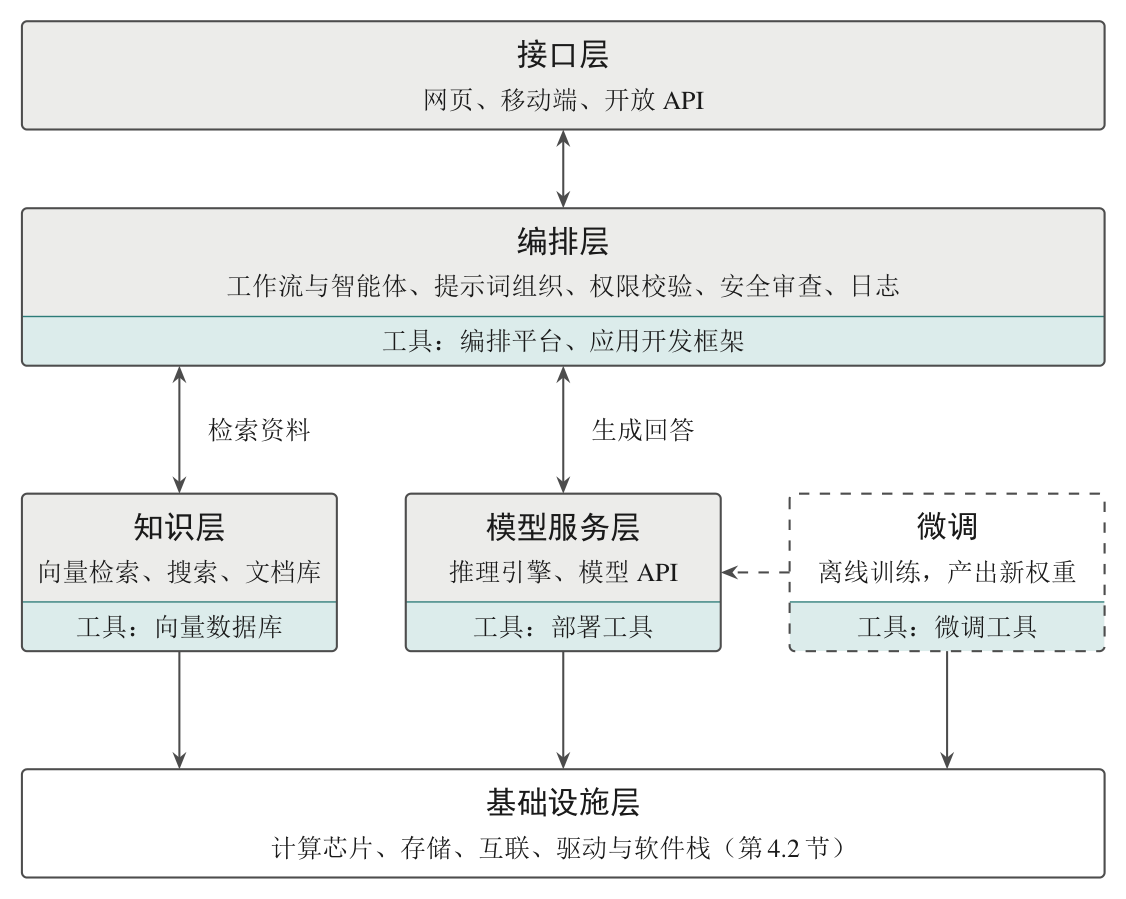
\includegraphics[width=0.9\linewidth]{figs/fig11.png}
\caption{图 4-11　 大模型应用的典型分层与五类工具的位置。每个框底部的色带标出该层对应的工具类别。编排层发起检索与模型调用；微调（虚线框）在线下进行，产出的权重交给模型服务层加载}
\end{figure}

\subsection*{4.5.2　 五类工具的定位}


根据所负责的链路，常用工具可分为五类（表\,4-6）。需要注意，这是按\textbf{功能定位}划分的分类，而非严格互斥的技术分类：许多产品同时具备多种能力。例如，某个部署工具既能管理模型，也能对外提供 API；某个编排平台既能搭建知识库，也能集成智能体。选型时应先明确工具负责哪一段链路，再比较具体产品。

\begin{table}[htbp]
\centering
\caption{表 4-6　 五类应用系统工具的定位}

\begin{tabular}{l l l l}
\toprule
类型 & 代表工具 & 主要功能 & 容易混淆之处 \\
\midrule
编排平台 & Coze、Dify、FastGPT、MaxKB & 可视化搭建工作流、接入知识库、发布应用 & 不是训练或计算框架 \\
应用开发框架 & LangChain、LlamaIndex、LangGraph & 以代码连接模型、工具与数据，实现控制逻辑 & 不提供算力，也不运行模型 \\
向量数据库 & Milvus、Faiss、Pinecone、Weaviate & 向量存储、近似最近邻检索、元数据过滤 & 只负责检索，不能代替模型生成回答 \\
微调工具 & LLaMA-Factory、Transformers + PEFT、XTuner、Unsloth & 组织数据与训练配置，支持 LoRA 等方法 & 与驱动、编译器不在同一层 \\
部署工具 & Ollama、LM Studio、vLLM、SGLang、TGI & 加载模型、执行推理、提供 API & “方便运行”与“高并发吞吐”是不同目标 \\
\bottomrule
\end{tabular}
\end{table}

\subsection*{4.5.3　 部署工具：本地运行与高并发服务}


部署工具可以按目标分为两类。

\paragraph{面向易用的本地运行工具} \textbf{Ollama} 是开源的跨平台工具，一条命令（如 \texttt{ollama run <模型名>}）即可下载并运行模型，提供兼容 OpenAI 格式的 REST API，并通过量化等手段使模型能够在个人电脑的 CPU 或 GPU 上运行。\textbf{LM Studio} 则提供图形界面，便于浏览、下载和试用模型。这类工具降低了模型部署运行的门槛，但它们不会改变模型的参数量和知识截止时间，也不会提升模型本身的能力。部分工具支持导入在其他工具中微调好的权重，但这并不等于工具本身完成了微调训练。

\paragraph{面向吞吐的推理引擎} \textbf{vLLM}、\textbf{SGLang}、TGI 等推理引擎面向多用户在线服务，其核心是第\,4.4.3\,小节介绍的技术：PagedAttention 管理 KV 缓存，连续批处理调度请求，并集成高效注意力内核与量化支持\cite{kwon2023vllm}。llama.cpp 则以 C/C++ 实现、对 CPU 和消费级硬件友好，常作为本地工具的底层引擎。

二者的取舍可以概括为：面向个人体验、离线开发和小规模试用时，优先考虑易用的本地工具；面向多用户并发、关注吞吐与尾延迟的生产服务时，应选用推理引擎，并按第\,4.4.4\,小节的方法实测。

\subsection*{4.5.4　 编排、检索与微调工具}

\paragraph{编排平台与应用开发框架} \textbf{LangChain} 等应用开发框架以代码形式连接模型、工具和数据源，用“链”或“图”组织多步流程；\textbf{Coze}、Dify 等低代码平台则通过可视化节点搭建问答、审批和知识库等业务流程。流程设计中有一个重要的权衡\cite{anthropic2024agents}：对于步骤固定、重复执行的任务，采用预先定义的\textbf{工作流}（{workflow}）更便于测试和管控；对于目标多变、步骤难以预先确定的任务，可引入能够自主选择工具、规划步骤的\textbf{智能体}（{agent}），同时必须设置权限边界和停止条件。智能体并非自主性越高越好，自主性越高，出错的代价和外部副作用通常也越大。

\paragraph{向量数据库与检索增强} 在检索增强生成（RAG）应用中，文档先被切分成片段，用嵌入模型转换为向量后存入向量数据库；用户提问时，系统检索与问题最相似的片段，交给模型参考作答。\textbf{Milvus} 是开源的分布式向量数据库，支持海量向量与元数据的存储、多种索引和相似性检索，采用存储与计算分离的云原生架构\cite{milvus2024}；Faiss 则是一个向量相似性检索\textbf{库}，需要嵌入到其他系统中使用，在部署和扩展方式上与完整的数据库不同。需要注意，向量相似并不等于事实正确，实际系统通常还要结合关键词检索、重排序、文档权限控制和回答评估。

\paragraph{微调工具} \textbf{LLaMA-Factory} 等工具将数据处理、训练配置、LoRA/QLoRA 等参数高效微调方法\cite{hu2021lora,dettmers2023qlora}以及评估导出集成在一起，并提供网页界面，降低了实验管理的门槛。但它们仍然依赖底层框架和硬件，并不会消除优化器状态和激活值带来的开销。要判断一个微调任务能否在单卡上完成，仍需按第\,4.3.3\,小节的方法，根据显存、量化方式、训练精度、批大小和序列长度进行估算。

\begin{quote}
\textbf{辨析}　 
“先微调还是先做 RAG”取决于要解决的问题。如果痛点是知识需要频繁更新、回答需要给出出处，RAG 通常是成本更低的起点；如果痛点是输出风格、特殊格式或特定任务行为，才进一步考虑微调。二者也可以结合使用。
\end{quote}

\begin{quote}
\textbf{本节要点}


\begin{itemize}[leftmargin=1.5em]
  \item “运行模型”只是大模型应用的一个环节，完整的产品还需要接口、编排、知识和基础设施。
  \item 五类工具按负责的链路区分；选型时先确定链路，再比较产品。
  \item 本地运行工具追求易用，推理引擎追求吞吐；工作流追求可控，智能体追求灵活。
\end{itemize}
\end{quote}

\section*{4.6　 综合案例：课程知识问答助手的系统设计}


\begin{quote}

\noindent 假设要为一门课程搭建知识问答助手，它既要能解释课程概念，又要给出讲义出处。该怎么搭、需要什么硬件、速度够不够？本节按自上而下的顺序回答：业务需求决定服务指标，服务指标决定模型与推理引擎，模型与负载决定显存和带宽需求，最后才确定硬件。每一步都先用本章的估算公式判断方案是否可行，再用实测验证并迭代。
\end{quote}

本节把前面各节的知识串联起来，完整演示一次系统设计。设计的顺序与本章的组织思路一致：\textbf{先明确需求，再选择方案，最后评估效果}（图\,4-12）。

\begin{figure}
\centering
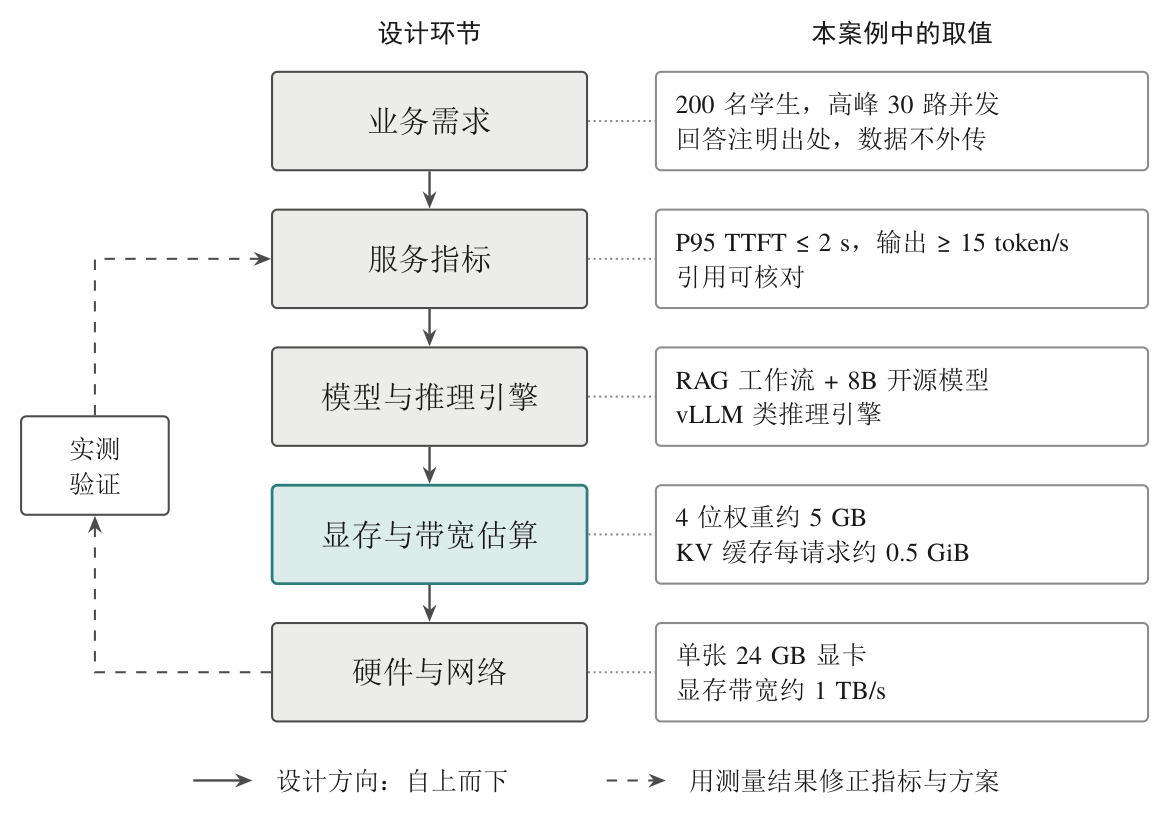
\includegraphics[width=0.9\linewidth]{figs/fig12.png}
\caption{图 4-12　 自上而下的系统设计流程及其在课程知识问答助手中的取值。高亮的估算环节决定了方案能否成立}
\end{figure}

\subsection*{4.6.1　 第一步：明确需求与服务指标}

某高校希望为一门课程开发问答助手，基本情况如下：
\begin{itemize}
  \item \textbf{用户与负载}：选课学生约 200 人，考试前的高峰时段约有 30 人同时提问；
  \item \textbf{数据}：课件和讲义共约 2000 页，每学期更新；
  \item \textbf{功能}：回答需注明出自哪份讲义的哪一页，便于学生核对；
  \item \textbf{约束}：课程资料不得上传到外部服务，预算为一台配备单张 \SI{24}{GB} 消费级显卡的服务器。
\end{itemize}

将需求转化为可度量的服务指标：P95 的 TTFT 不超过 \SI{2}{s}；输出速度不低于每秒 15 个 token（明显快于阅读速度）；在 30 路并发下服务保持稳定；引用页码的正确率需通过人工抽查评估。

\subsection*{4.6.2　 第二步：自上而下选择方案}

\paragraph{应用层：先 RAG，不微调} 需求的核心是“知识准确且可溯源”，而且资料每学期更新，这正是 RAG 擅长的任务（见第\,4.5\,节的辨析）。因此不需要训练或微调模型。处理流程固定为：解析讲义并保存课程、讲次、页码等元数据；对问题同时做向量检索和关键词检索；把检索到的片段与问题一起交给模型；生成带引用的回答。由于步骤固定，采用工作流而非智能体，便于测试和排错。2000 页资料切分后约为数万个片段，规模很小，单机向量库即可满足需求。

\paragraph{模型层：选择规模与精度} 数据不能外传，因此在本地部署开源权重模型。考虑到显存只有 \SI{24}{GB}，选择约 8B 参数的指令模型。由式\,\eqref{eq:weight-mem} 估算：BF16 权重约 \SI{16}{GB}，4 位量化后约 \SI{5}{GB}（含元数据）。

\paragraph{服务层：选择推理引擎} 高峰期有 30 路并发，需要连续批处理和高效的 KV 缓存管理，因此选用 vLLM 一类的推理引擎，而不是以单用户体验为主的本地运行工具。

\subsection*{4.6.3　 第三步：估算效果，检查可行性}

\paragraph{显存是否够用} 每个请求的上下文按 4096 个 token 计（问题、检索片段与回答之和），由例\,4-3 估算，每个请求的 KV 缓存约 \SI{0.5}{GiB}。扣除运行时开销（按约 \SI{2}{GB} 计）后：
\begin{itemize}
  \item BF16 权重：剩余约 \SI{6}{GB}，仅能容纳约 11 个请求，\textbf{无法满足} 30 路并发；
  \item 4 位量化权重：剩余约 \SI{17}{GB}，可容纳约 31 个请求，\textbf{基本满足}需求，但余量很小。
\end{itemize}
因此选择 4 位量化。若实测发现回答质量明显下降，可以考虑缩短检索上下文、对 KV 缓存也进行量化，或者增加一张显卡。

\paragraph{速度是否够快} 该显卡的显存带宽约 \SI{1}{TB/s}。按第\,4.1.2\,小节的方法，4 位权重下单请求解码速度的理论上限约为 $1000/5=200$ token/s。即便实际只能达到上限的几分之一，且多个请求共享带宽，也有较大把握满足每秒 15 个 token 的目标。预填充阶段，3000 个输入 token 约需 $2\times8\times10^{9}\times3000\approx5\times10^{13}$ 次浮点运算，按有效算力约 $10^{14}$\,FLOP/s 计，耗时约 \SI{0.5}{s}，满足 TTFT 目标；高峰期的排队时间则需要实测确认。

\paragraph{瓶颈可能在哪里} 以上估算表明，在这个场景中，主要约束是\textbf{显存容量}（决定并发上限），而不是峰值算力。如果实测发现响应慢的主要原因在检索环节，就应优化索引和重排序，而不是更换显卡。

\subsection*{4.6.4　 第四步：实测验证}

估算只能判断方案大致是否可行，最终必须以实测为准。建议开展以下三项实验：
\begin{enumerate}
  \item \textbf{单请求基线}：固定输出长度，分别使用 512、2048、4096 个 token 的输入，记录 TTFT 与输出速度，检验预填充时间随输入长度的变化；
  \item \textbf{并发压力测试}：保持模型、硬件和提示词不变，把并发数从 1 逐步增加到 40，绘制总吞吐与 P95 延迟随并发的变化曲线，找出 KV 缓存耗尽、开始排队的拐点；
  \item \textbf{检索效果检验}：向索引中加入或移除一份带页码的讲义，观察回答内容与引用是否随之变化，并人工抽查引用的正确率。
\end{enumerate}
实验报告应记录硬件型号、驱动与引擎版本、模型与量化方式、输入输出长度分布和并发设置，确保结果可以复现。

\begin{quote}
\textbf{本节要点}


这个案例体现了本章的核心思路：\textbf{业务需求决定服务指标，服务指标决定模型与推理引擎，模型与负载决定存储与带宽需求，存储、带宽与并发需求最终决定硬件和网络}。只记住工具的名称，无法完成这样的设计；掌握各层的作用与估算方法，才能在动手之前判断方案是否可行。
\end{quote}

\section*{4.7　 本章小结与展望}


本章以“大模型需要什么”为线索，依次讨论了计算系统各层如何满足这些需求。回顾全章：
\begin{itemize}
  \item \textbf{计算需求}回答“大模型要算多少、存多少、搬多少”：参数量、计算量和数据搬运量这三个基本量决定了计算系统的负担；Roofline 模型用于判断一项计算受算力限制还是受访存限制（第\,4.1\,节）。
  \item \textbf{算力资源}回答“计算在哪里执行、数据如何存取和传输”：芯片提供算力，HBM 提供容量与带宽，NVLink 和 InfiniBand 连接多卡多机，计算软件栈把硬件能力开放给上层（第\,4.2\,节）。
  \item \textbf{深度学习框架}回答“如何定义、训练和扩展计算”：自动微分将模型定义与计算执行分离开来，数据并行、张量并行、流水线并行与 ZeRO 用于解决单卡显存不足的问题（第\,4.3\,节）。
  \item \textbf{推理服务}回答“如何快速、低成本地服务大量请求”：预填充阶段计算受限，解码阶段访存受限；KV 缓存、FlashAttention、PagedAttention、连续批处理与量化分别作用于推理过程的不同环节（第\,4.4\,节）。
  \item \textbf{应用系统工具}回答“如何把模型变成可用、可管理的产品”：部署、微调、检索、开发框架与编排平台各自负责一段链路（第\,4.5\,节）。
\end{itemize}

展望未来，大模型计算系统的发展并非仅靠把芯片做得更大，而是多个层次的协同演进：更低精度的数值格式与相应的编译优化，更灵活的显存与缓存管理，更高效的片内与片间互联，面向超大集群的调度与容错，对国产芯片等异构硬件的统一支持，以及面向长时间运行的智能体任务的安全服务边界。理解各层之间的约束关系，比学会调用某一个模型 API 更接近可迁移的工程能力。

\section*{习题}



\begin{enumerate}[label=\thechapter.\arabic*,leftmargin=2.6em,itemsep=4pt]
  \item （估算）一个 13B 参数的模型，分别以 BF16、INT8 和 4 位精度存储时，模型权重各约占多少 GB？为什么实际运行需要更多显存？
  \item （Roofline）某 GPU 峰值算力为 \SI{300}{TFLOP/s}，显存带宽为 \SI{1.5}{TB/s}。求其拐点算术强度。批大小为 1 的解码阶段与长输入的预填充阶段，分别落在 Roofline 的哪个区域？
  \item （概念）两块显卡的 FP16 峰值算力接近，但运行同一个 7B 模型时，单请求的输出速度相差明显。请列出至少三种可能的原因。
  \item （概念）PCIe、NVLink 和 InfiniBand 分别位于数据通路的哪个层次？RDMA 与它们是什么关系？
  \item （计算）按 BF16 混合精度与 Adam 的配置，估算 13B 模型全参数训练所需的模型状态显存；若使用 16 张卡并采用 ZeRO-3，每张卡约需多少显存？
  \item （辨析）普通数据并行与 ZeRO-3 在显存占用上的根本区别是什么？ZeRO-3 的代价是什么？
  \item （计算）某模型有 40 层，KV 头数为 8，每头 128 维，以 BF16 存储 KV 缓存。若要在 \SI{40}{GB} 的可用显存中同时处理 20 个请求，每个请求的序列长度最多为多少？
  \item （辨析）为什么采用连续批处理通常能提高总吞吐，却不能保证每个请求的 TTFT 都降低？
  \item （设计）为企业内部的知识助手进行选型时，应优先考虑微调还是 RAG？请说明判断依据。
  \item （设计）参照第\,4.6\,节，为“200 人同时在线的编程作业答疑助手”给出一个自上而下的设计方案，并指出最可能成为瓶颈的环节。
\end{enumerate}

\subsection*{部分习题提示}
\begin{small}
\begin{description}[leftmargin=2.6em, labelwidth=2.2em, font=\normalfont]
  \item[4.1] 由式\,\eqref{eq:weight-mem}，BF16 约 \SI{26}{GB}，INT8 约 \SI{13}{GB}，4 位约 \SI{6.5}{GB}。实际运行还需存放量化元数据、KV 缓存、运行时缓冲区和临时张量。
  \item[4.2] $I^{*}=300\times10^{12}/1.5\times10^{12}=200$\,FLOP/byte。批大小为 1 的解码阶段 $I\approx1$，访存受限；长输入的预填充阶段 $I\approx T$，输入足够长时计算受限。
  \item[4.3] 可从显存带宽、内核实现效率、KV 缓存读取效率、批大小以及是否发生 CPU 卸载等方面分析。
  \item[4.5] 模型状态约 $13\times10^9\times16\approx\SI{208}{GB}$；ZeRO-3 下每卡约 $208/16=\SI{13}{GB}$，另需激活值与通信缓冲区。
  \item[4.7] 每 token 每请求的 KV 缓存为 $2\times40\times8\times128\times2=\SI{163840}{B}$，则 $T\le 40\times10^{9}/(20\times163840)\approx 12\,200$。
  \item[4.8] 考虑多个请求共享资源导致的排队、调度顺序和 KV 缓存占用。
\end{description}
\end{small}

\section*{本章术语}



{\begin{longtable}{lll}
\toprule
缩写/术语 & 英文全称 & 中文 \\
\midrule
\endhead
ASIC & Application-Specific Integrated Circuit & 专用集成电路 \\
CPU / GPU / NPU & Central / Graphics / Neural Processing Unit & 中央/图形/神经网络处理器 \\
HBM & High Bandwidth Memory & 高带宽内存 \\
TSV & Through-Silicon Via & 硅通孔 \\
PCIe & Peripheral Component Interconnect Express & 高速外设互联总线 \\
RDMA & Remote Direct Memory Access & 远程直接内存访问 \\
RoCE & RDMA over Converged Ethernet & 基于以太网的 RDMA \\
Roofline & Roofline Model & 屋顶线模型 \\
DP / TP / PP / EP & Data / Tensor / Pipeline / Expert Parallelism & 数据/张量/流水线/专家并行 \\
ZeRO & Zero Redundancy Optimizer & 零冗余优化器 \\
FSDP & Fully Sharded Data Parallel & 全分片数据并行 \\
KV Cache & Key-Value Cache & 键值缓存 \\
TTFT & Time To First Token & 首 token 延迟 \\
TPOT & Time Per Output Token & 每 token 输出时间 \\
GQA / MQA & Grouped-Query / Multi-Query Attention & 分组查询/多查询注意力 \\
RAG & Retrieval-Augmented Generation & 检索增强生成 \\
LoRA & Low-Rank Adaptation & 低秩适配 \\
\bottomrule
\end{longtable}
}

\begin{thebibliography}{99}
\bibitem{zhao2024llm} 赵鑫, 李军毅, 周昆, 唐天一, 文继荣. 大语言模型[M]. 北京: 高等教育出版社, 2024.

\bibitem{zhang2023d2l} Zhang A, Lipton Z C, Li M, Smola A J. Dive into Deep Learning[M]. Cambridge: Cambridge University Press, 2023. \url{https://d2l.ai}

\bibitem{goodfellow2016deep} Goodfellow I, Bengio Y, Courville A. Deep Learning[M]. Cambridge, MA: MIT Press, 2016.

\bibitem{hwu2026pmpp} Hwu W W, Kirk D B, El Hajj I. Programming Massively Parallel Processors: A Hands-on Approach[M]. 5th ed. Cambridge, MA: Morgan Kaufmann, 2026.

\bibitem{kaplan2020scaling} Kaplan J, McCandlish S, Henighan T, et al. Scaling Laws for Neural Language Models[EB/OL]. arXiv:2001.08361, 2020.

\bibitem{williams2009roofline} Williams S, Waterman A, Patterson D. Roofline: An Insightful Visual Performance Model for Multicore Architectures[J]. Communications of the ACM, 2009, 52(4): 65--76.

\bibitem{nvidia2023h100} NVIDIA. NVIDIA H100 Tensor Core GPU Datasheet[EB/OL]. 2023. \url{https://www.nvidia.com/en-us/data-center/h100/}

\bibitem{nvidia2024cuda} NVIDIA. CUDA C++ Programming Guide[EB/OL]. \url{https://docs.nvidia.com/cuda/cuda-c-programming-guide/}

\bibitem{paszke2019pytorch} Paszke A, Gross S, Massa F, et al. PyTorch: An Imperative Style, High-Performance Deep Learning Library[C]//Advances in Neural Information Processing Systems 32. 2019: 8024--8035.

\bibitem{ansel2024pytorch2} Ansel J, Yang E, He H, et al. PyTorch 2: Faster Machine Learning Through Dynamic Python Bytecode Transformation and Graph Compilation[C]//Proceedings of ASPLOS. 2024: 929--947.

\bibitem{rajbhandari2020zero} Rajbhandari S, Rasley J, Ruwase O, He Y. ZeRO: Memory Optimizations Toward Training Trillion Parameter Models[C]//Proceedings of SC20. 2020: 1--16.

\bibitem{shoeybi2019megatron} Shoeybi M, Patwary M, Puri R, et al. Megatron-LM: Training Multi-Billion Parameter Language Models Using Model Parallelism[EB/OL]. arXiv:1909.08053, 2019.

\bibitem{hu2021lora} Hu E J, Shen Y, Wallis P, et al. LoRA: Low-Rank Adaptation of Large Language Models[EB/OL]. arXiv:2106.09685, 2021.

\bibitem{dettmers2023qlora} Dettmers T, Pagnoni A, Holtzman A, Zettlemoyer L. QLoRA: Efficient Finetuning of Quantized LLMs[EB/OL]. arXiv:2305.14314, 2023.

\bibitem{dao2022flashattention} Dao T, Fu D Y, Ermon S, et al. FlashAttention: Fast and Memory-Efficient Exact Attention with IO-Awareness[C]//Advances in Neural Information Processing Systems 35. 2022.

\bibitem{kwon2023vllm} Kwon W, Li Z, Zhuang S, et al. Efficient Memory Management for Large Language Model Serving with PagedAttention[C]//Proceedings of SOSP. 2023: 611--626.

\bibitem{yu2022orca} Yu G I, Jeong J S, Kim G W, et al. Orca: A Distributed Serving System for Transformer-Based Generative Models[C]//Proceedings of OSDI. 2022: 521--538.

\bibitem{milvus2024} Milvus. What is Milvus?[EB/OL]. \url{https://milvus.io/docs/overview.md}

\bibitem{anthropic2024agents} Anthropic. Building Effective Agents[EB/OL]. 2024. \url{https://www.anthropic.com/research/building-effective-agents}

\end{thebibliography}

\end{document}
